% Number 730
% UCM SFriction Algebra Units Vectors
% Banked curve
% JG

% Watermark
\AddToShipoutPicture*{\BackgroundPic}

\addtocounter {ProbNum} {1}

%\begin{floatingfigure}[r]{.42\textwidth}
%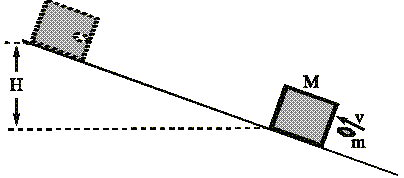
\includegraphics[scale=.6]{/Users/jgates/desktop/latex/pics/inclinebulletblock}
%\end{floatingfigure}
 
{\bf \Large{\arabic{ProbNum}}} A car rounds a curve with a radius of 50 meters.  The curve is banked 15 degrees.

\bigskip
Determine the speed at which a car could round the curve without the assistance of friction - if the road were covered in ice, what one speed would allow the car to safely make the turn?\paragraph{}
\noindent
\vfill

Determine the coefficient of static friction necessary for the car to round the curve twice as fast as the "design speed" found above.
\vfill

\vfill
%\hfill 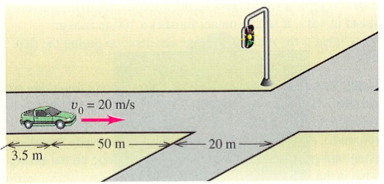
\includegraphics[scale=.85]{/Users/jgates/desktop/latex/pics/redlight.png}
\newpage